%----------------------------------------------------------
\chapter*{ВВЕДЕНИЕ}\label{ch:introduction}
\addcontentsline{toc}{chapter}{ВВЕДЕНИЕ}

%-------------------------------------------------------

В современном программировании становится все более важным сколько будет потрачено времени на создание того или иного продукта.
В это число входит как время, потраченное непосредственно на создание приложения, так и время, потраченное на его поддержку.
Поэтому инструменты, применяемые программистом в повседневной работе, должны всячески помочь ему в этом.

Пожалуй, самым главным таким инструментом является компилятор.
Разработчики компиляторов прикладывают большие усилия, чтобы язык программирования отвечал требованиям надежности и скорости.
При создании инструмента такого рода важно правильно выбирать и проектировать каждую часть.
Одной из основных таких частей является то, как в языке программирования взаимодействуют друг с другом типы.

В высокоуровневых языках программирования типы окружают разработчика повсюду.
Чем более развитая система типов, там больше можно выразить, используя ее, а значит, если она надежна и подкреплена математической основой, то в программе станет меньше ошибок.
Кроме того, в таком случае программы можно будет применять в качестве доказательств для различных теорий~\cite{AutoProvement}.
Сейчас такое уже применяет компания Intel при проектировании новых алгоритмов умножения или деления.

Актуальна проблема высокого порога входа в некоторые функциональные языки программирования, например Haskell и др.
Он завышен, так как в них применяются сложные математические теории, повлиявшие и на синтаксис языка, и на всю его идеологию в целом.
Поэтому появилась идея создать язык программирования, вобравший в себя идеи функциональных языков, но при этом сохранивший C-подобный синтаксис.
Кроме того, он задумывался еще и как способ изучить всю цепочку создания компилятора.
На сегодняшний день уже разработан синтаксис языка (листинг~\ref{lst:syntax}), стабилизировано его внутреннее представление (\textit{абстрактное синтаксическое дерево (AST)}), а также ведется работа над компилятором.

Абстрактным синтаксическим деревом называют структуру данных, получаемую после синтаксического анализа.
В ней связываются элементы синтаксиса языка: параметры функции, объявление переменной и т.д.

\begin{lstlisting}[label={lst:syntax},caption={Демонстрация синтаксиса языка Kodept}]
    module Main =>
    fun greeting(name: String) => "Hello " + name + "!"
    fun main => print(greeting("world"))
\end{lstlisting}

Компилятор в языке программирования обычно разделен на несколько частей (рис. \ref{fig:pipeline}).
Одной из них является семантический анализ.
В него входят анализ областей видимости объявлений, \textit{проверка (и вывод) типов} и др.

Проверкой типов называют процесс, когда тем или иным образом проверяется правильность типа выражения согласно системе типов языка.
В ходе научно-исследовательской работы была выбрана система типов Хиндли-Милнера.
Алгоритм W~\cite{UrbanN2009}, реализующий ее, позволяет также проводить вывод типов.

\begin{figure}[H]
    \centering
    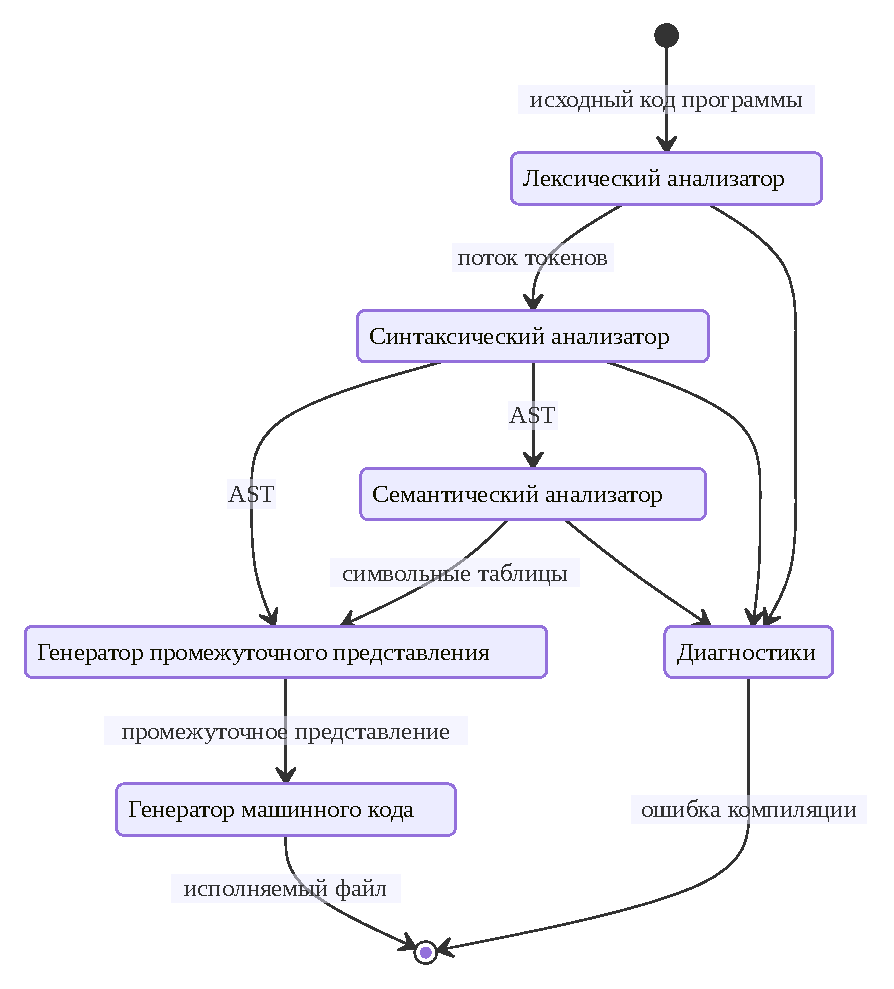
\includegraphics[width=0.75\textwidth]{figures/pipeline}
    \caption{Схема состояний работы компилятора}
    \label{fig:pipeline}
\end{figure}

\textbf{Целью} курсового проекта является реализация механизма вывода и проверки типов для языка программирования Kodept в качестве его дальнейшего развития.

%----------------------------------------------------------
